\section{Triggers}

\def\figpath{figures/nr-int-note/trigger/V1/}

This analysis uses a combination of multi \Pqb-jet triggers. 
The \pt thresholds and \Pqb-tagging working points vary slightly by the year of data taking ( with the specific cut values delineated in \Tab{\ref{tab:nr-triggers}}).
note - only 2 \Pqb-tags are required in the trigger to avoid creating a bias in the control region used in the background estimation that will be described in \Sect{\ref{sec:rw-overview}}.
The \Pqb-tagging SFs are derived for each trigger chain individually required our analysis strategy to specify which trigger stream was considered for the trigger SF application.
One other interesting feature of our analysis is our signal is not fully efficient for our analysis, as illustrated by efficiencies that are less than 100\% in Fig{\ref{fig:HH_trigger_eff}}, and also this efficiency is varying as a function of the reconstructed 4-jet invariant mass. 
 
\begin{table}[htbp]
\centering
\begin{tabular}{p{2cm}  p{1cm} | p{6cm}  | p{4.5cm} }
\textbf{Trigger Type} & Year & HLT thresholds & L1 thresholds \\
\hline
{} & 2016 & \small{ $\pt > 100$~GeV jet \& two $\pt > 55$~GeV 60\%~WP \Pqb-jets } &  \small{ five $\pt > 15$~GeV jets} \\
\textbf{2b1j} & 2017 &  \small{ $\pt > 150$~GeV jet \& two $\pt > 55$~GeV 70\%~WP \Pqb-jets }&  \small{ $\pt > 85$~GeV jet \& two $\pt~>~30$~GeV jets } \\
{} & 2018 &  \small{ $\pt > 150$~GeV jet \& two $\pt > 55$~GeV 70\%~WP \Pqb-jets }&  \small{ $\pt > 85$~GeV jet \& two $\pt~>~30$~GeV jets }\\
\hline
{} & 2016 &  \small{ four $\pt > 35$~GeV jets, two 60\% WP \Pqb-tags} & {} \\ 
\textbf{2b2j} & 2017 &  \small{four  $\pt > 35$~GeV jets, two 40\% WP \Pqb-tags} &  \small{four $\pt > 15$~GeV,  $|\eta| < 2.5$ jets} \\
{} &  2018 &  \small{four $\pt > 35$~GeV jets, two 60\% WP \Pqb-tags}  & {} \\
\end{tabular}
\caption{Triggers used for non-resonant searches. For \Pqb-tagging in the trigger in Run 2, the MV2 version of the \Pqb-tagger is used. Also, an L1 $|\eta| < 3.2$ cut is assumed where not specified.}
\label{tab:nr-triggers}
\end{table}

\begin{figure}[htb]
        \centering
                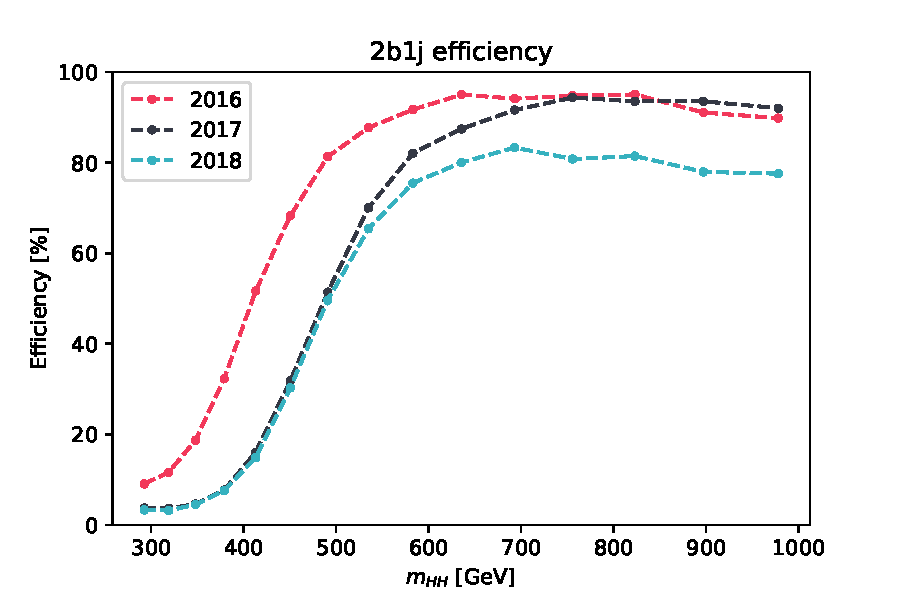
\includegraphics[width=0.32\textwidth]{\figpath/SMNR_ggF_600043-2b1j-trigger-efficiency.pdf}
                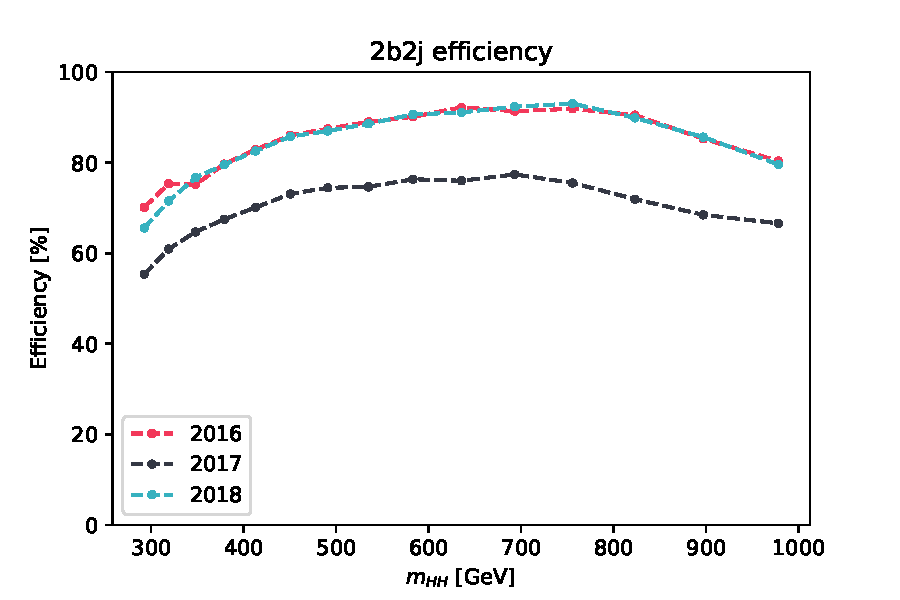
\includegraphics[width=0.32\textwidth]{\figpath/SMNR_ggF_600043-2b2j-trigger-efficiency.pdf}
                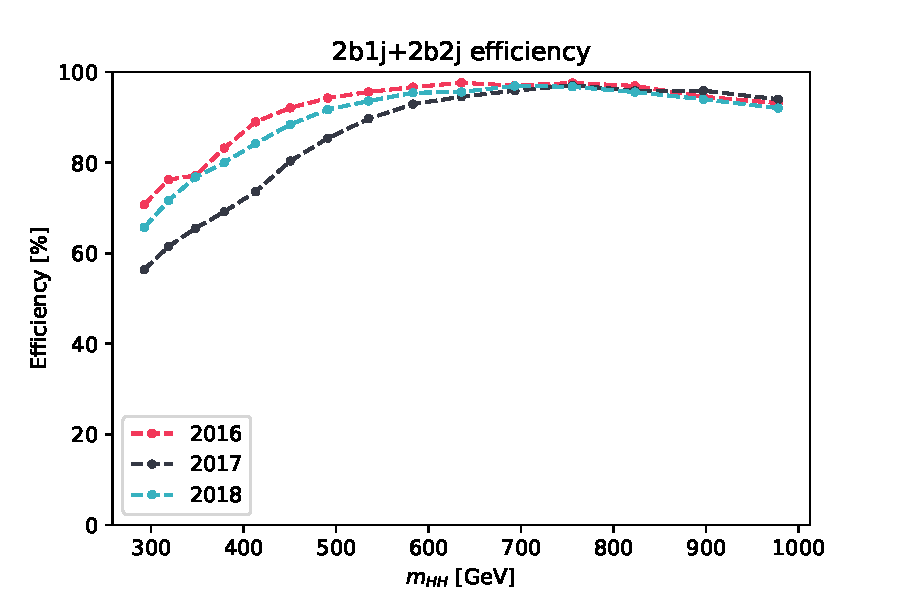
\includegraphics[width=0.32\textwidth]{\figpath/SMNR_ggF_600043-2b1j+2b2j-trigger-efficiency.pdf}
        \caption{Trigger efficiencies of the 2b1j, 2b2j and combined for the MC16a/d/e corresponding to years 2016-2018 for the SM ggF \kl=1 signal.
        Significantly lower efficiency for 2017 2b2j comparing to other years is due to tighter b-tagging requirement (lower efficiency). \hl{Is this plot inside of the SR?}}
	\label{fig:HH_trigger_eff}
\end{figure}

To account for this feature of ``operating on the turn on curve'' the SF that we apply to account for the trigger effects 

%%%%%%%%%%%%%%%%%%%%%%%%%%%%%%%
\subsection{Trigger buckets}
%%%%%%%%%%%%%%%%%%%%%%%%%%%%%%%

To distinguish which trigger chain to check, we cut on the offline jets $p_{\text{T},1} > 170$~GeV and $p_{\text{T},3} > 70$~GeV, where the jets are ordered by \pt.
These jet \pt cuts mimic the 2b1j trigger.
If the event passes these jet cuts, we put it in trigger \textbf{bucket 1}, otherwise it goes in trigger \textbf{bucket 2}.
In trigger bucket 1, we check the decision of the 2b1j trigger to decide whether to keep the event, and in trigger bucket 2, we check the 2b2j trigger. This procedure is summarized graphically in \Fig{\ref{fig:trigger-bucket-strategy}}.

\begin{figure}[htbp]
    \centering
    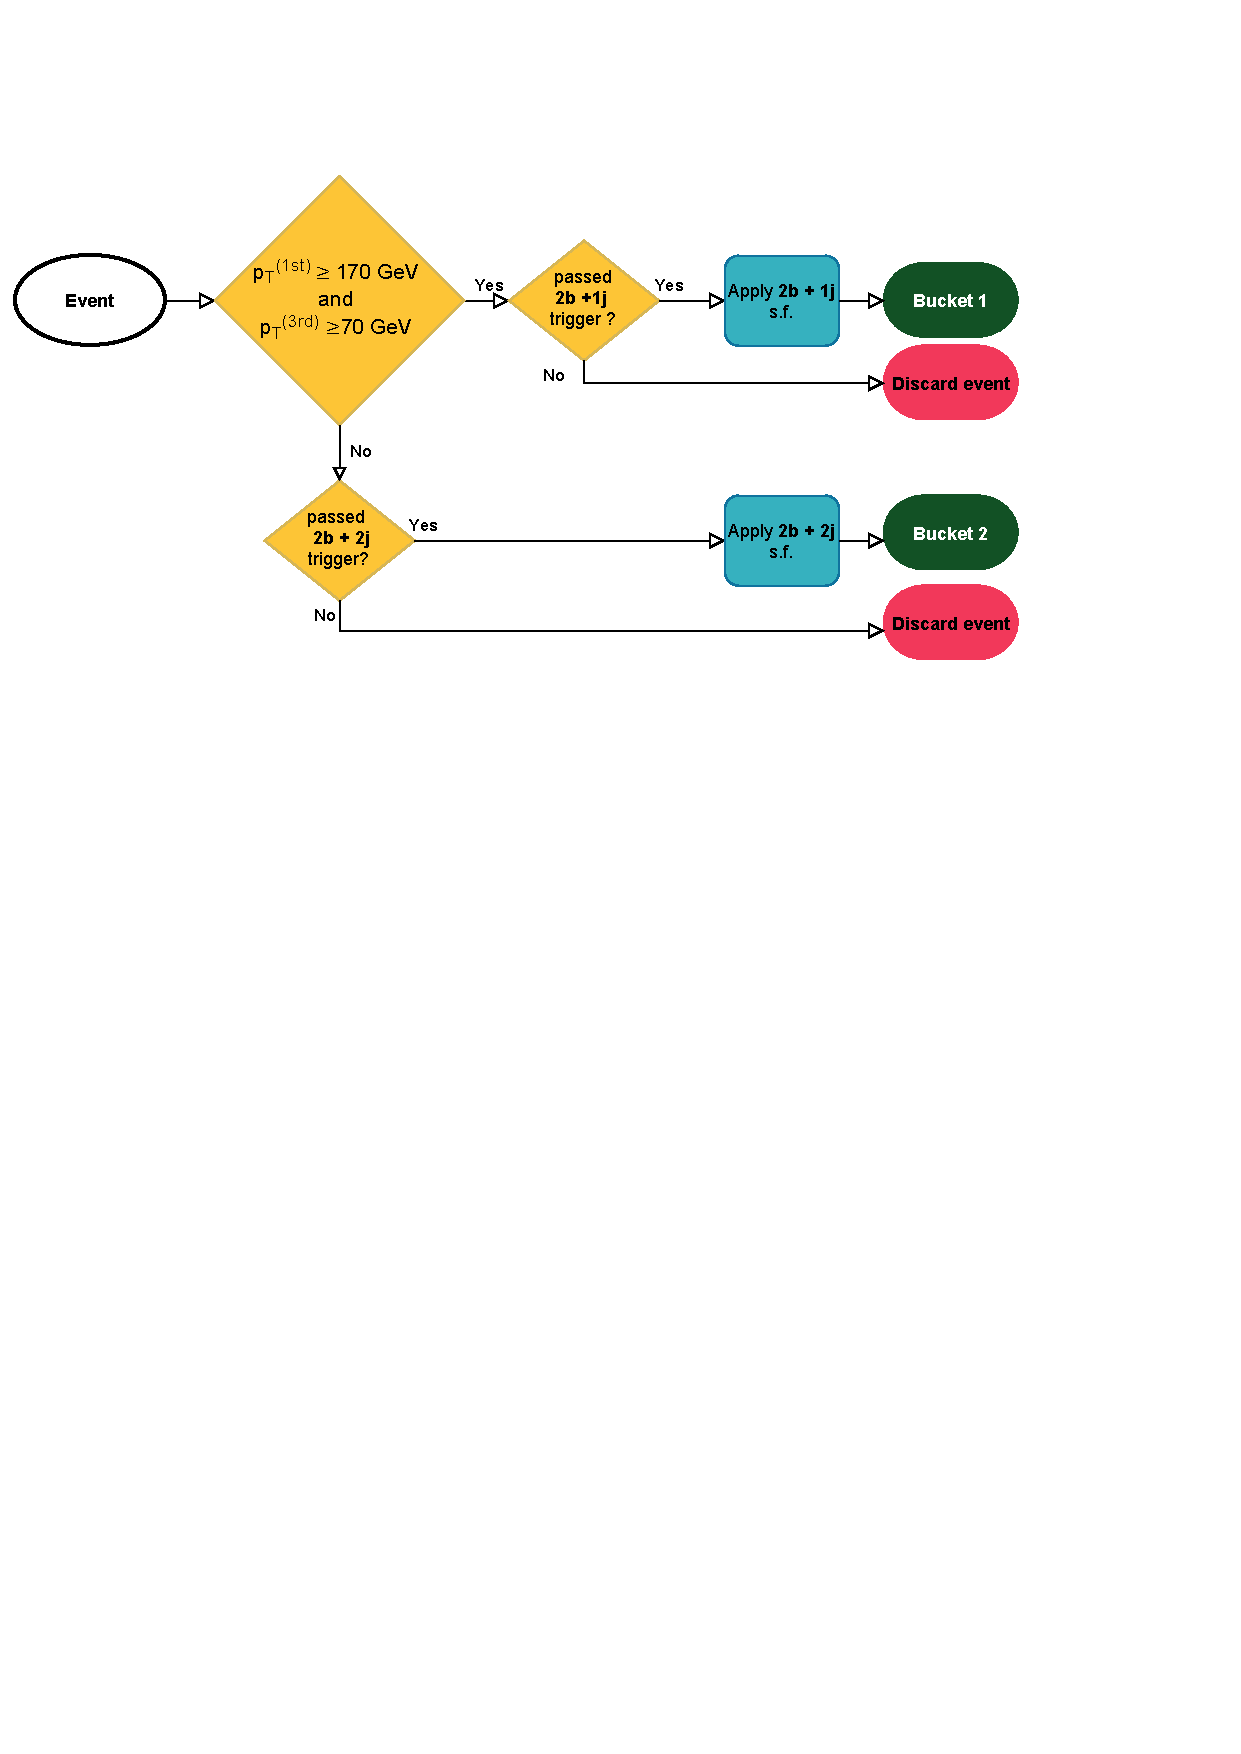
\includegraphics[width=0.8\textwidth]{\figpath/nr_buckets_diagram_simple.pdf}
    \caption{Trigger bucket strategy for non-resonant searches.}
    \label{fig:trigger-bucket-strategy}
\end{figure}

\Fig{\ref{fig:trig-bucket-4b}} shows how this strategy of using a combination of two triggers gives us sensitivity to complementary phase spaces in the analysis. The 2b1j trigger drives our acceptance for the high \mhh events, while the 2b2j trigger provides our low \mhh acceptance.

\begin{figure}
    \centering
    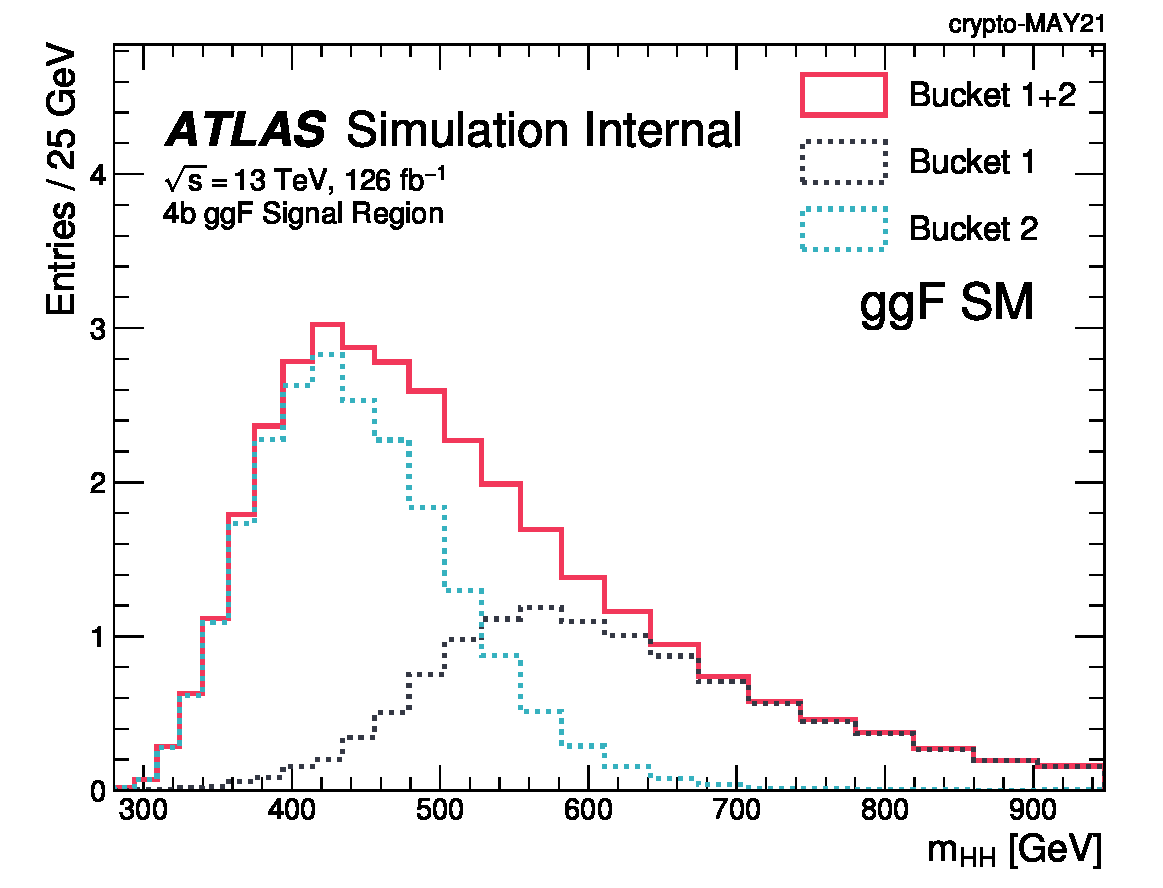
\includegraphics[width=0.48\textwidth]{\figpath/buckets_comparison_4b_ggF_SM_SR.pdf}
    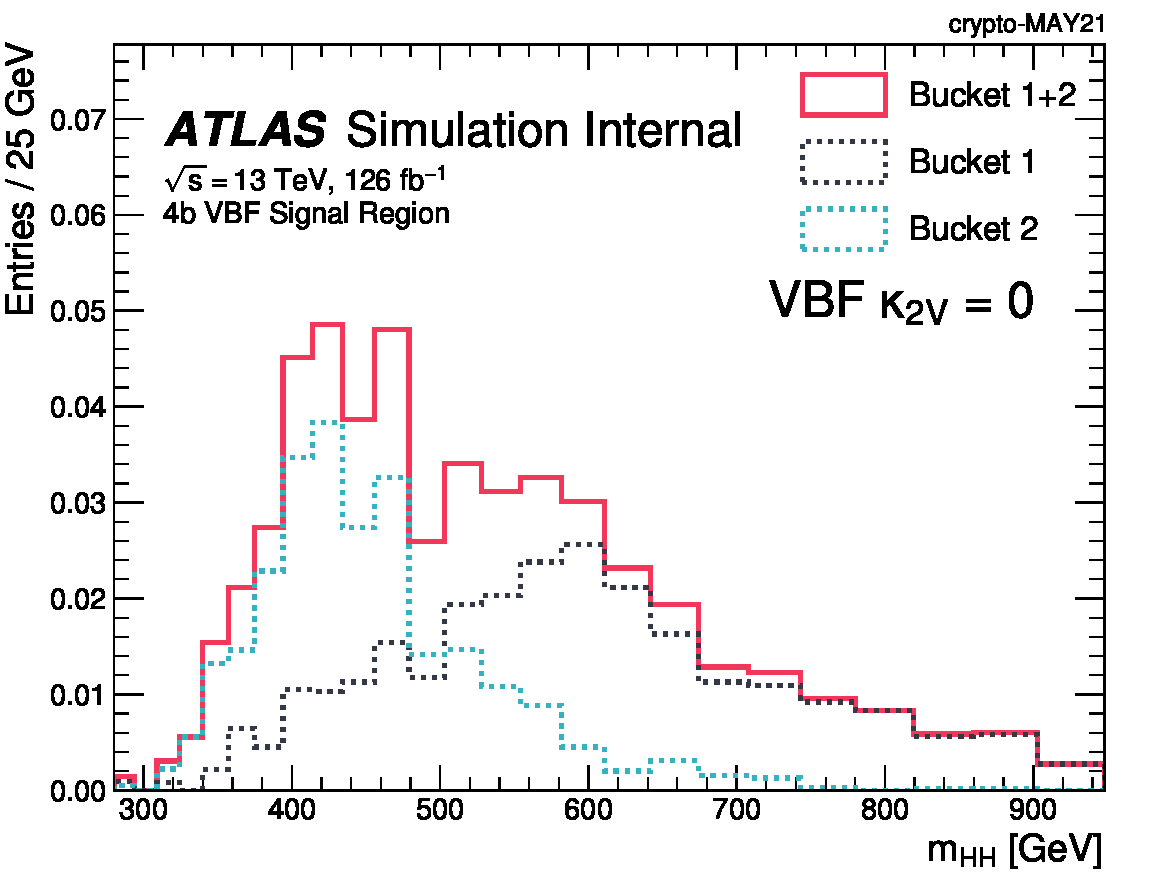
\includegraphics[width=0.48\textwidth]{\figpath/buckets_comparison_4b_VBF_SR.pdf}
    \caption{The bucket composition of \mhh for the SM ggF (left) and \kvv = 0 VBF (right) \HH MC simulation in the 4b Signal Regions.  Bucket 1 corresponds to the 2b1j trigger and Bucket 2 corresponds to the 2b2j trigger.}
    \label{fig:trig-bucket-4b}
\end{figure}

To reconstruct the trigger decision and define the jet level SFs, offline jets are matched to the online jets using a $\Delta R$matching criterion.
% There are different cuts being used:
% - dR < 0.4 for defining the trigger match and applying the CDI SFs
% - dR < 0.3 for deriving the HLT ET SFs
% - dR < 0.4 for deriving the L1 ET SFs
% but I'm not sure if dR < 0.4 is always used for applying these SFs
These online jets are then checked to pass the (online) thresholds given in Table~2, and if this many jets and \Pqb-jets pass this selection, the event passes this trigger. 
For ease of knowing how to apply the SFs, we will only keep events where the trigger passed in the relevant bucket, i.e, the 2b1j trigger needs to pass if the event passed the offline cuts in bucket 2, and the 2b2j trigger needs to pass if the event passed the offline cuts in bucket 1.
The event level trigger SF is calculated from the jet level SFs (\Eq{\ref{eq:trig-sf-all}}) with two contributions:

\begin{equation}
\text{Multi \Pqb-jet trigger SF} = \prod_i \textcolor{dodgerblue}{  SF_{jet}^{b-tag}(i)} \times \textcolor{orange}{SF_{jet}^{kinematic}(i)}  
\label{eq:trig-sf-all}
 \end{equation}

\begin{itemize}
\item \textcolor{dodgerblue}{ \Pqb-jet trigger SFs using prescription from by the \Pqb-jet trigger group (described in \Sect{\ref{subsec:trig-sf-bjet}})}
%(although they were customly rederived down to 30 GeV since we were investigating a low \pT category).}
\item  \textcolor{orange}{ Kinematic $E_\text{T}$ HLT and L1 SFs derived in a custom $t\bar{t}$ analysis (described in \Sect{\ref{subsec:trig-sf-et}})}
\end{itemize}

%%%%%%%%%%%%%%%%%%%%%%%%%%%%%%%
\subsection{b-jet SF}
\label{subsec:trig-sf-bjet}
%%%%%%%%%%%%%%%%%%%%%%%%%%%%%%%

The offline and online \Pqb-tagging decisions are highly correlated, so the online \Pqb-tagging SF are derived conditional based on the offline \Pqb-tagging decision. 
Since both the offline and online $\Pqb$-tagging decisions could pass or fail, this gives four cases:

\begin{itemize}
\setlength\itemsep{-1.5em}
   \item Case 1: Pass online and offline \Pqb-tagging: 
   	\vspace{-1em}
	  \begin{equation*}
		 \varepsilon(\text{on} \land \text{off}) 
		 = \varepsilon(\text{on} | \text{off}) \varepsilon(\text{off})
	  \end{equation*}
   \item Case 2: Fail the online \Pqb-tag, but pass the offline \Pqb-tag: 
   	\vspace{-1em}
	  \begin{equation*}
		 \varepsilon(\overline{\text{on}} \land \text{off}) 
		 = [1 - \varepsilon(\text{on} | \text{off})] \varepsilon(\text{off})
	  \end{equation*}
   \item Case 3: Pass the online \Pqb-tag, but fail the offline \Pqb-tag: 
   	\vspace{-1em}
	  \begin{equation*}
		 \varepsilon(\text{on} \land \overline{\text{off}}) 
		 = \varepsilon(\text{on}) - \varepsilon(\text{on} | \text{off}) \varepsilon(\text{off})
	  \end{equation*}
   \item Case 4: Fail the online and offline \Pqb-tagging: 
   	\vspace{-1em}
	  \begin{equation*}
		 \varepsilon(\overline{\text{on}} \land \overline{\text{off}}) 
		 = 1 - \varepsilon(\text{off}) - \varepsilon(\text{on}) + \varepsilon(\text{on} | \text{off}) \varepsilon(\text{off})
	  \end{equation*}
\end{itemize}

Then for each efficiency, we still apply $SF = \varepsilon^{data} / \varepsilon^{MC}$.
For offline jets that are not matched to a corresponding online HLT jet, just the offline SF is applied, just the offline \Pqb-tagging SF is applied, as visualized in \Fig{\ref{fig:ftag-online-sf}}.

\begin{figure}
\centering
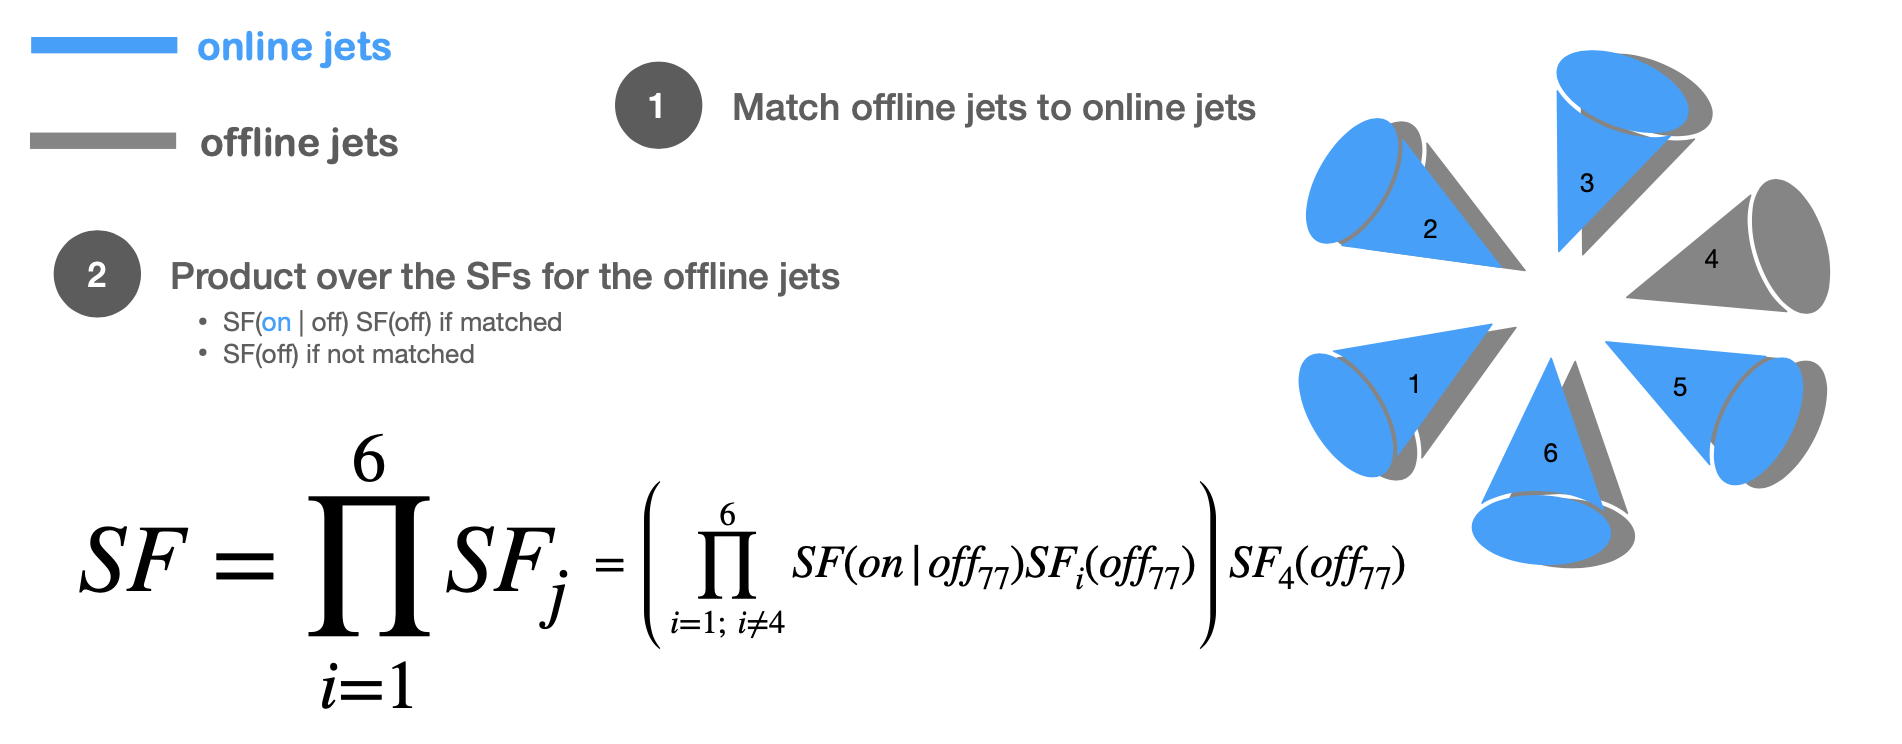
\includegraphics[width=\textwidth]{figures/my_dihiggs/check-btag-jets-sf.png}
\caption{Illustration of how the combined offline / online \Pqb-tagging SF is calculated.}
\label{fig:ftag-online-sf}
\end{figure}

Our use of the \Pqb-jet triggers dictates SFs dictates how much of the Run~2 dataset we can use.
\begin{enumerate}
\item In 2016 there was an issue in the online beam spot calculation, which impacted the primary vertex calculation for the HLT \Pqb-tagging. Because of this, we don't use this portion of the data from the 2016 dataset, a loss of 8.3~\ifb from the 32.8~\ifb of the full 2016 dataset.
\item Even for 2017 and 2018, we need to discard the first luminosity blocks of data taking where the beam spot has not yet had time to update. This means analyses with \Pqb-jet triggers have $\approx 1.5$\% lower luminosity in these years than the baseline luminosity \cite{b-trig-paper}.
\item The astute reader might notice that the 2015 triggers are not included in \Tab{\ref{tab:nr-triggers}}. As will be explained in \Sect{ch:bkg-est}, the background estimate is derived for each year separately to account for the differences in the trigger, and the robustness of the background estimate is partially based on the size of the sample used to derive it. Since it wasn't clear whether the 2015 dataset was large enough to warrant the gains of the additional complexity in the analysis, the 2015 conditional \Pqb-jet trigger SFs were never derived with respect to the offline DL1r algorithm, so this year of data is not included.
%Although the 2015 data was included in the partial Run~2 analysis \cite{paper-4b-36ifb}, in the intervening years ATLAS revamped the offline \Pqb-tagging software - and the conditional online SFs were not rederived with respect to the online \Pqb-tagger.
\end{enumerate}

In summary, when accounting for the above three points, \Tab{\ref{tab:lumi-yr}} is the (by year) luminosity for the 4b analysis, with a total luminosity is 126.0~\ifb. %, $\approx 10$\% lower than the 139~\ifb for analyses that don't need \Pqb-jet triggers.

\begin{table}[htbp]
\centering
\begin{tabular}{| c | c |}
\hline
\textbf{Year} & \textbf{Luminosity}  [\ifb] \\
\hline
2016 & 24.6 \\
2017 & 43.7 \\
2018 & 57.7 \\
\hline
all & 126.0 \\
\hline
\end{tabular}
\caption{Luminosty (by year) for the 4b analysis.}
\label{tab:lumi-yr}
\end{table}

%%%%%%%%%%%%%%%%%%%%%%%%%%%%%%%
\subsection{Kinematic SF}
\label{subsec:trig-sf-et}
%%%%%%%%%%%%%%%%%%%%%%%%%%%%%%%

\hl{Q that I have -- how do we apply the jet level SFs? Do we multiply over all of the offline jets in the event, but these are only non-unary for the first $N$ jets ordered by online ET?}

\begin{figure}[ht]
    \centering
    \subfloat[1st jet at L1]{\label{fig:jet-level-trigSF17-2b1j-L1-1st}
            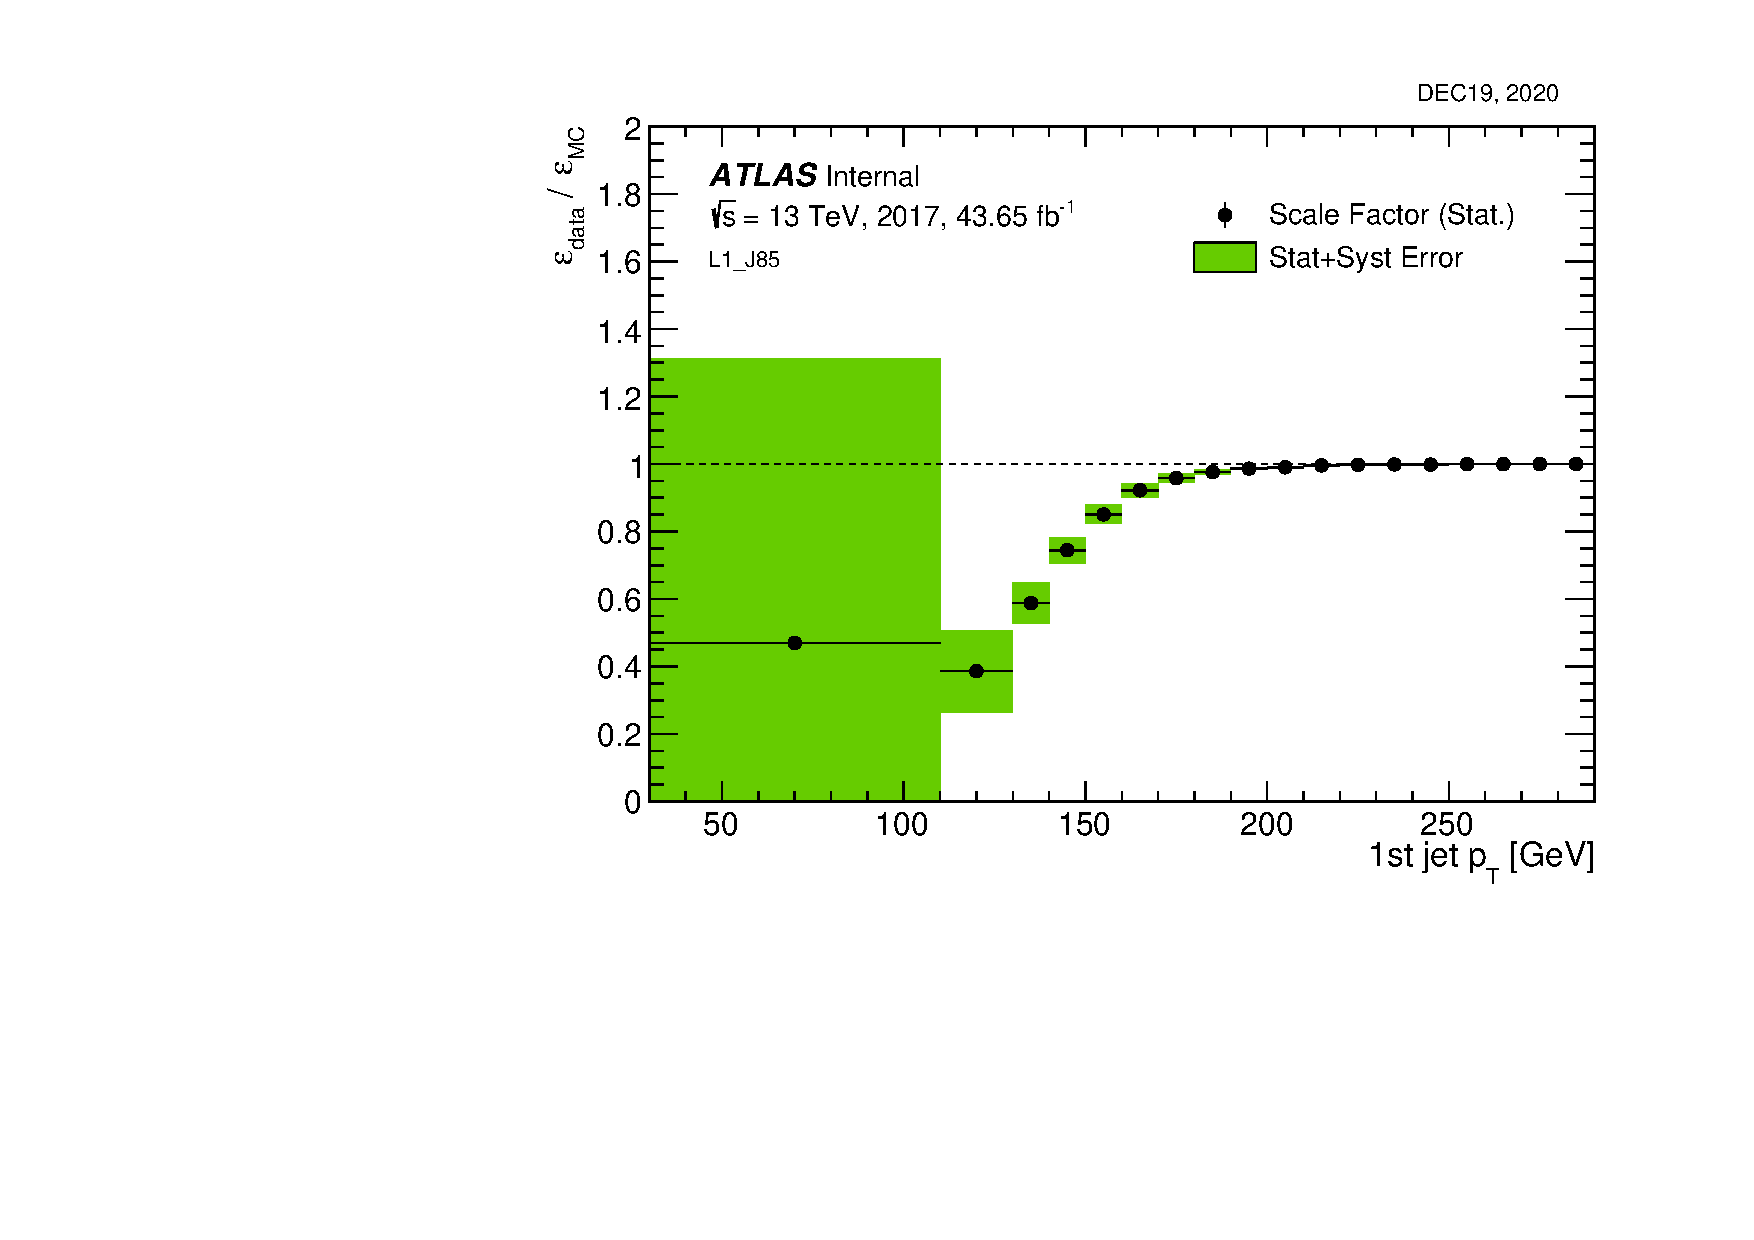
\includegraphics[width=0.3\textwidth]{figures/nr-int-note/appendices/jet-level-trigger-sf/V1/L1SF/2017/trigSF17-2b1j-L1-1st.pdf}
    }
    \subfloat[2nd jet at L1]{\label{fig:jet-level-trigSF17-2b1j-L1-2nd}
            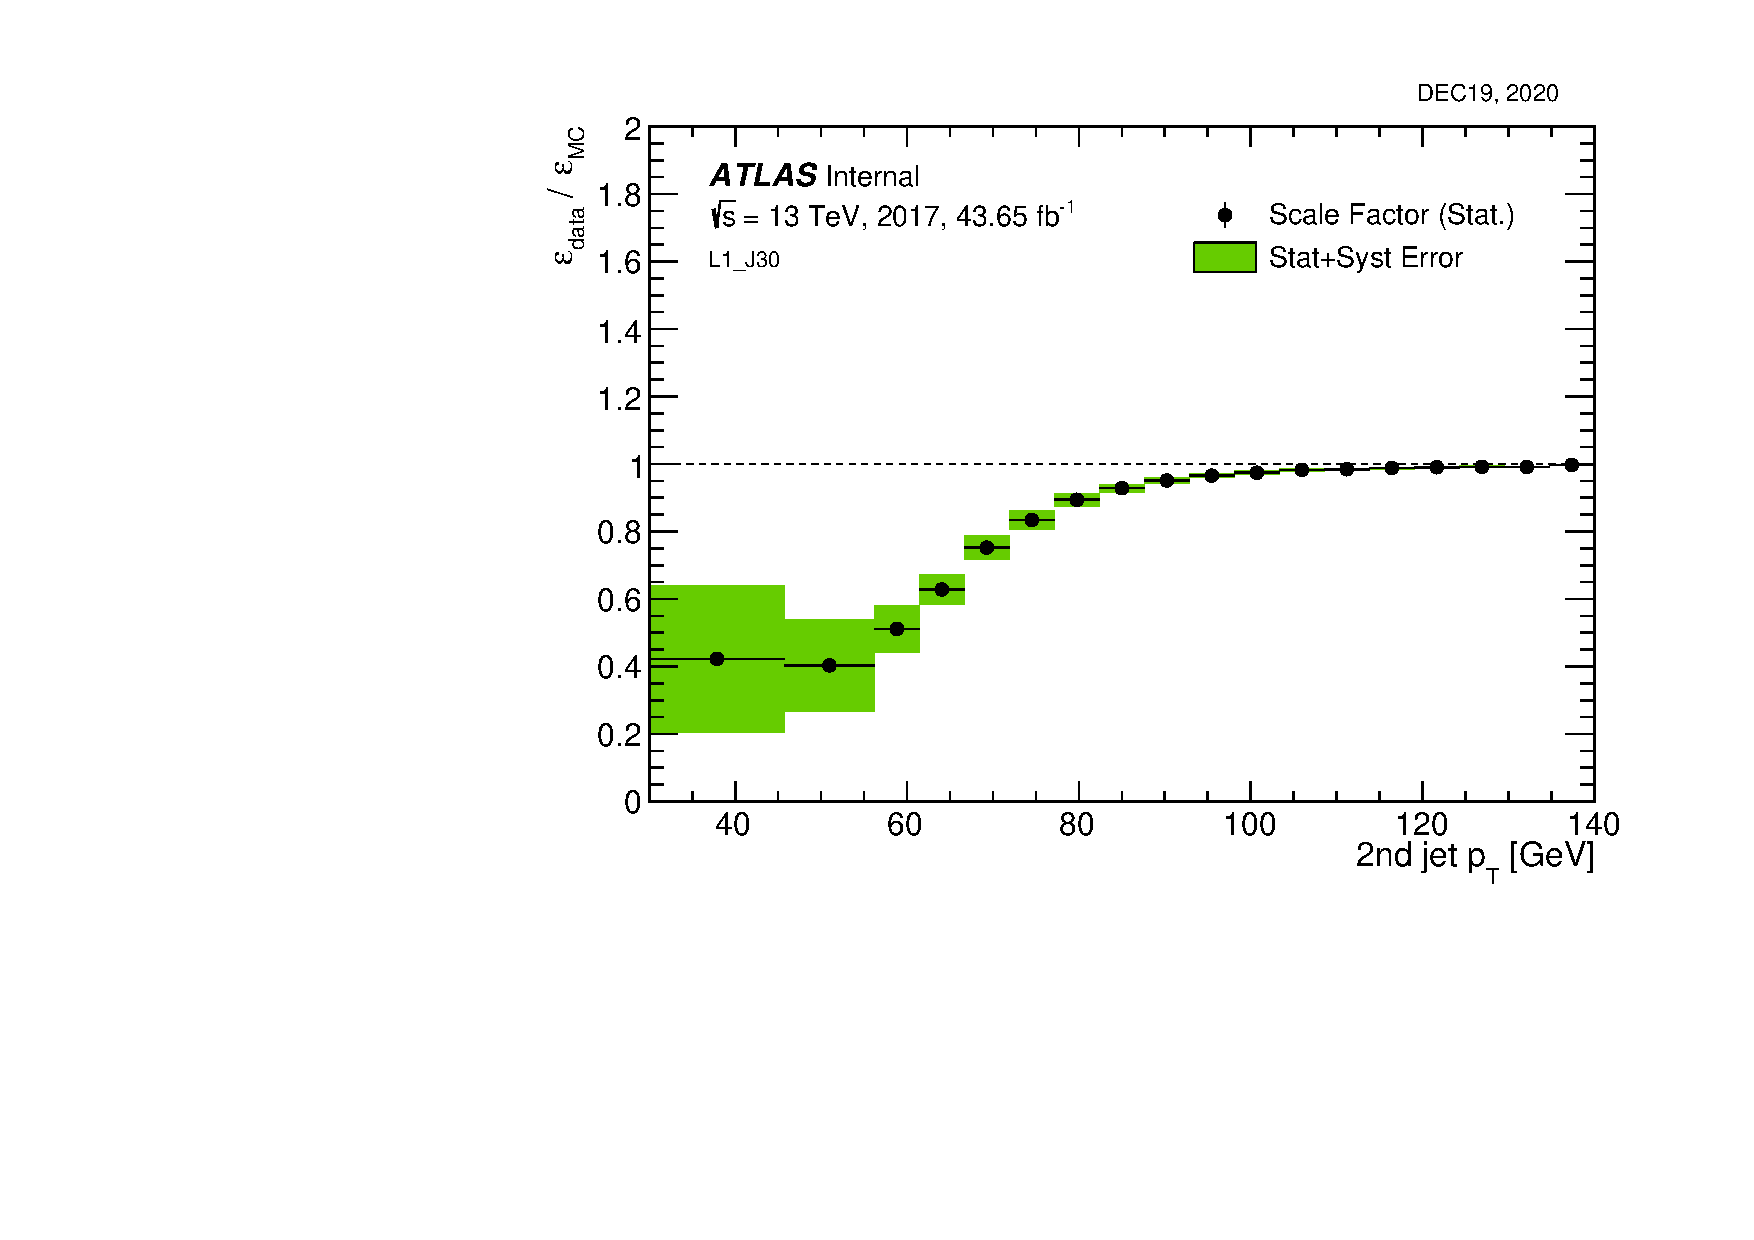
\includegraphics[width=0.3\textwidth]{figures/nr-int-note/appendices/jet-level-trigger-sf/V1/L1SF/2017/trigSF17-2b1j-L1-2nd.pdf}
    }
    \subfloat[3rd jet at L1]{\label{fig:jet-level-trigSF17-2b1j-L1-3rd}
            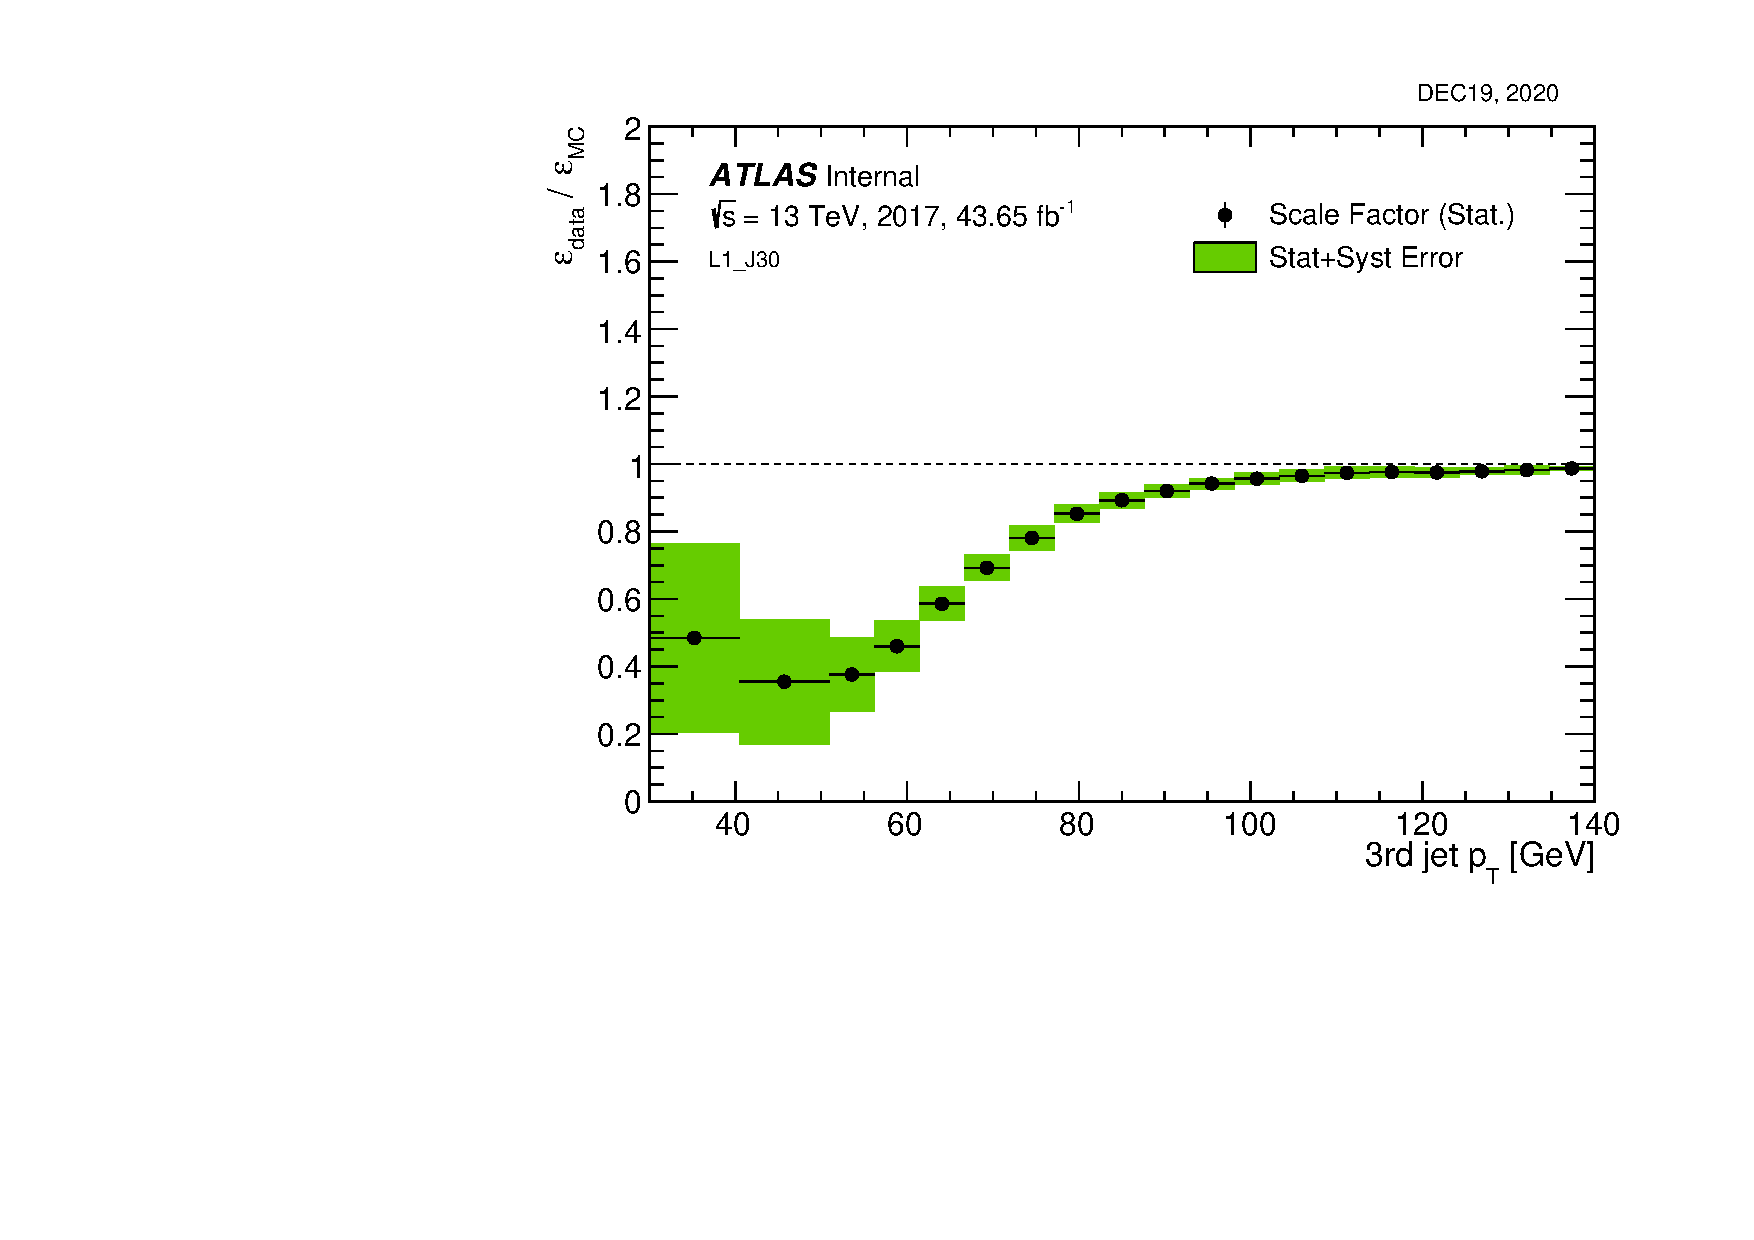
\includegraphics[width=0.3\textwidth]{figures/nr-int-note/appendices/jet-level-trigger-sf/V1/L1SF/2017/trigSF17-2b1j-L1-3rd.pdf}
    }

    \subfloat[1st jet at HLT]{\label{fig:jet-level-trigSF17-2b1j-HLT-1st}
            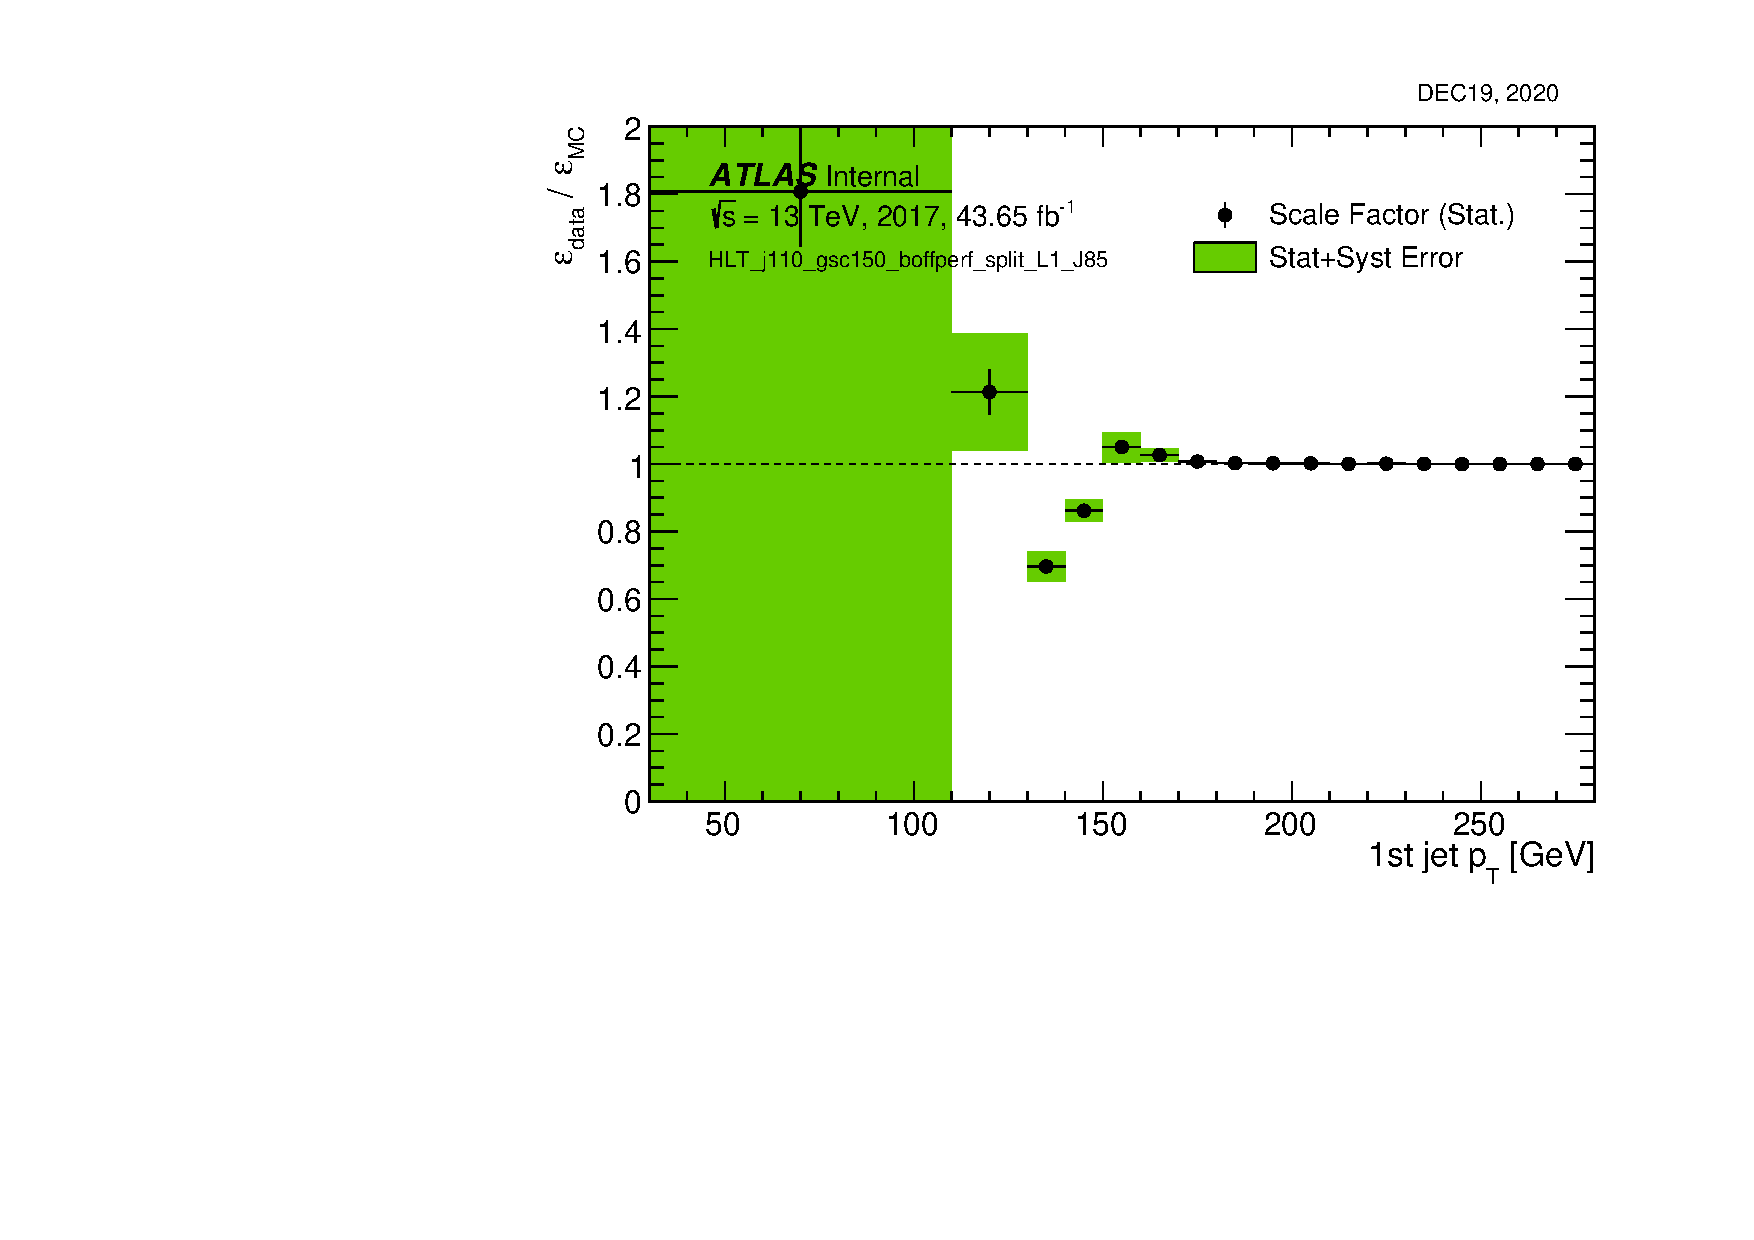
\includegraphics[width=0.3\textwidth]{figures/nr-int-note/appendices/jet-level-trigger-sf/V1/HLTSF/2017/trigSF17-2b1j-HLT-1st.pdf}
    }
    \subfloat[2nd jet at HLT]{\label{fig:jet-level-trigSF17-2b1j-HLT-2nd}
            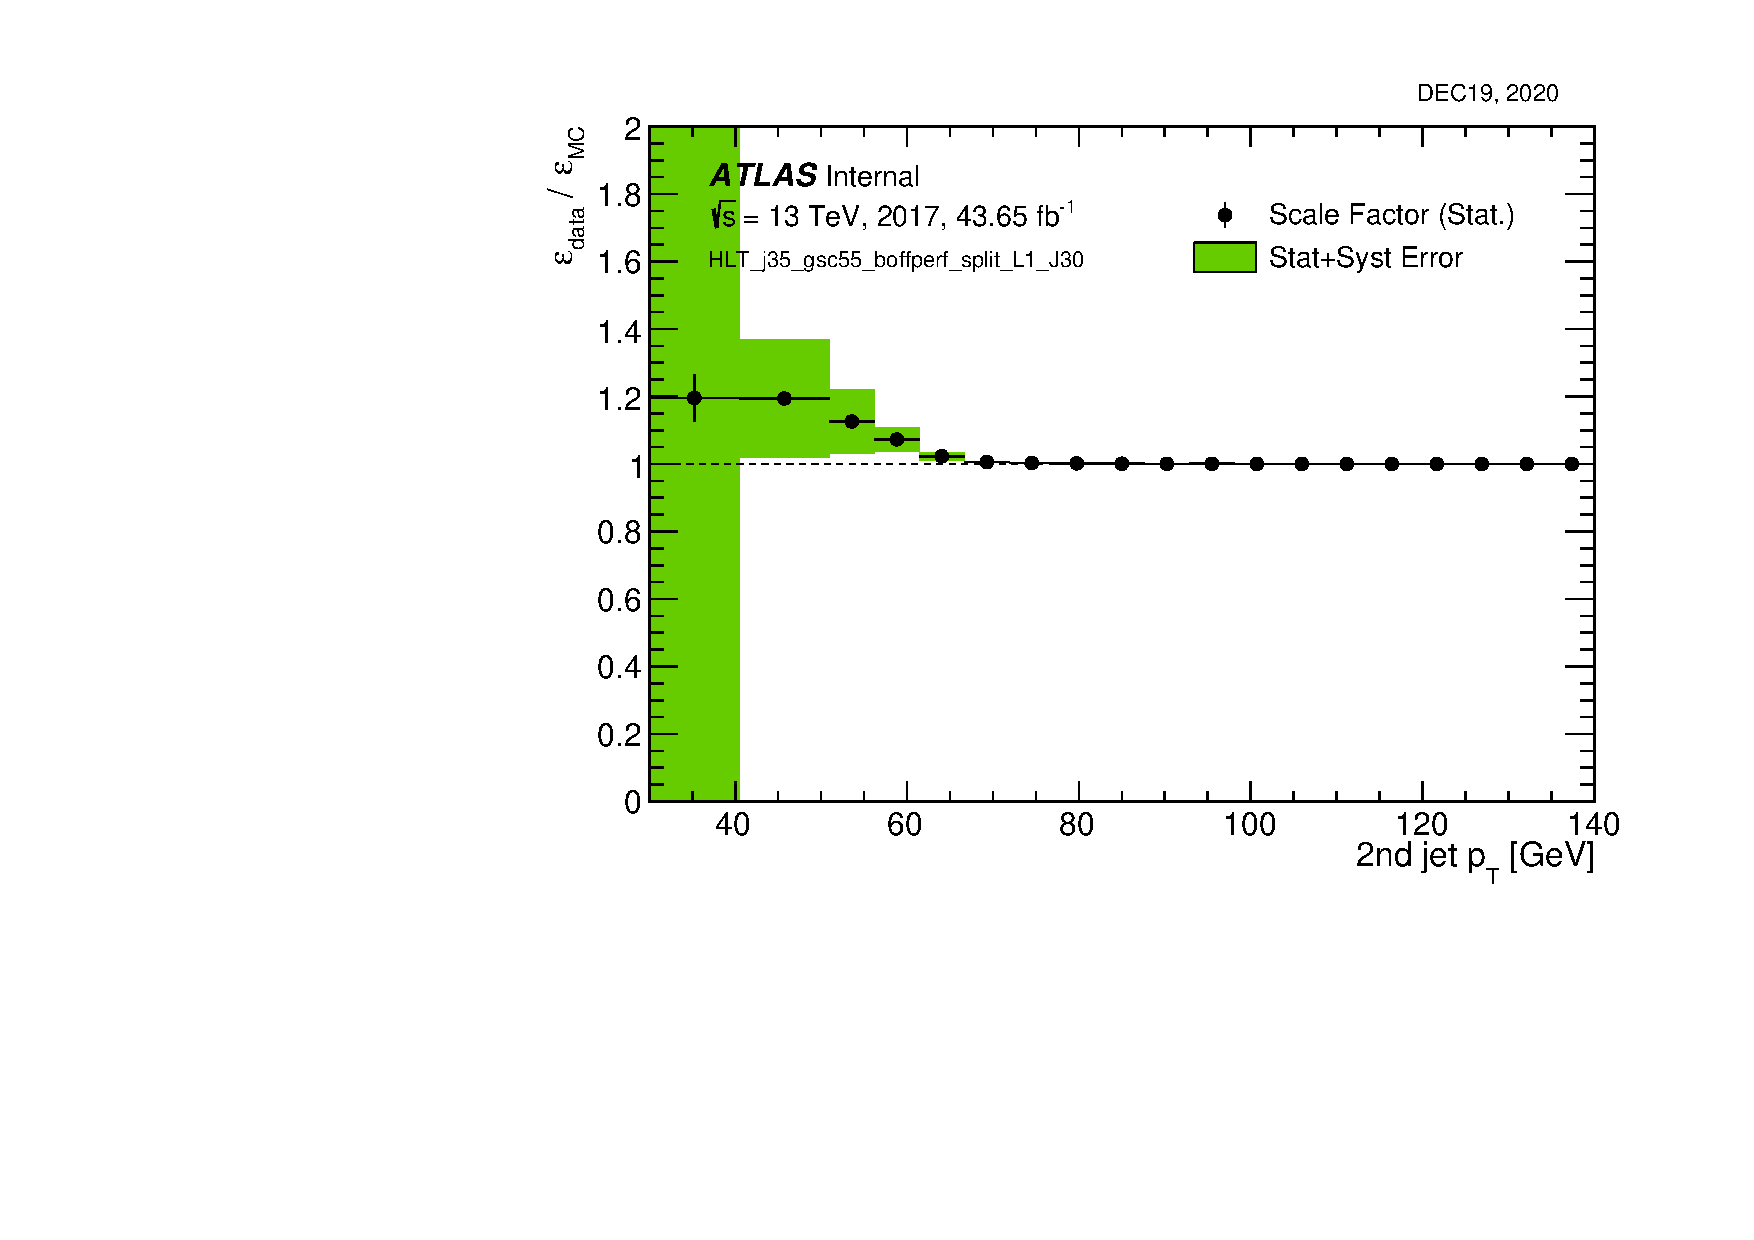
\includegraphics[width=0.3\textwidth]{figures/nr-int-note/appendices/jet-level-trigger-sf/V1/HLTSF/2017/trigSF17-2b1j-HLT-2nd.pdf}
    }
    \subfloat[3rd jet at HLT]{\label{fig:jet-level-trigSF17-2b1j-HLT-3rd}
            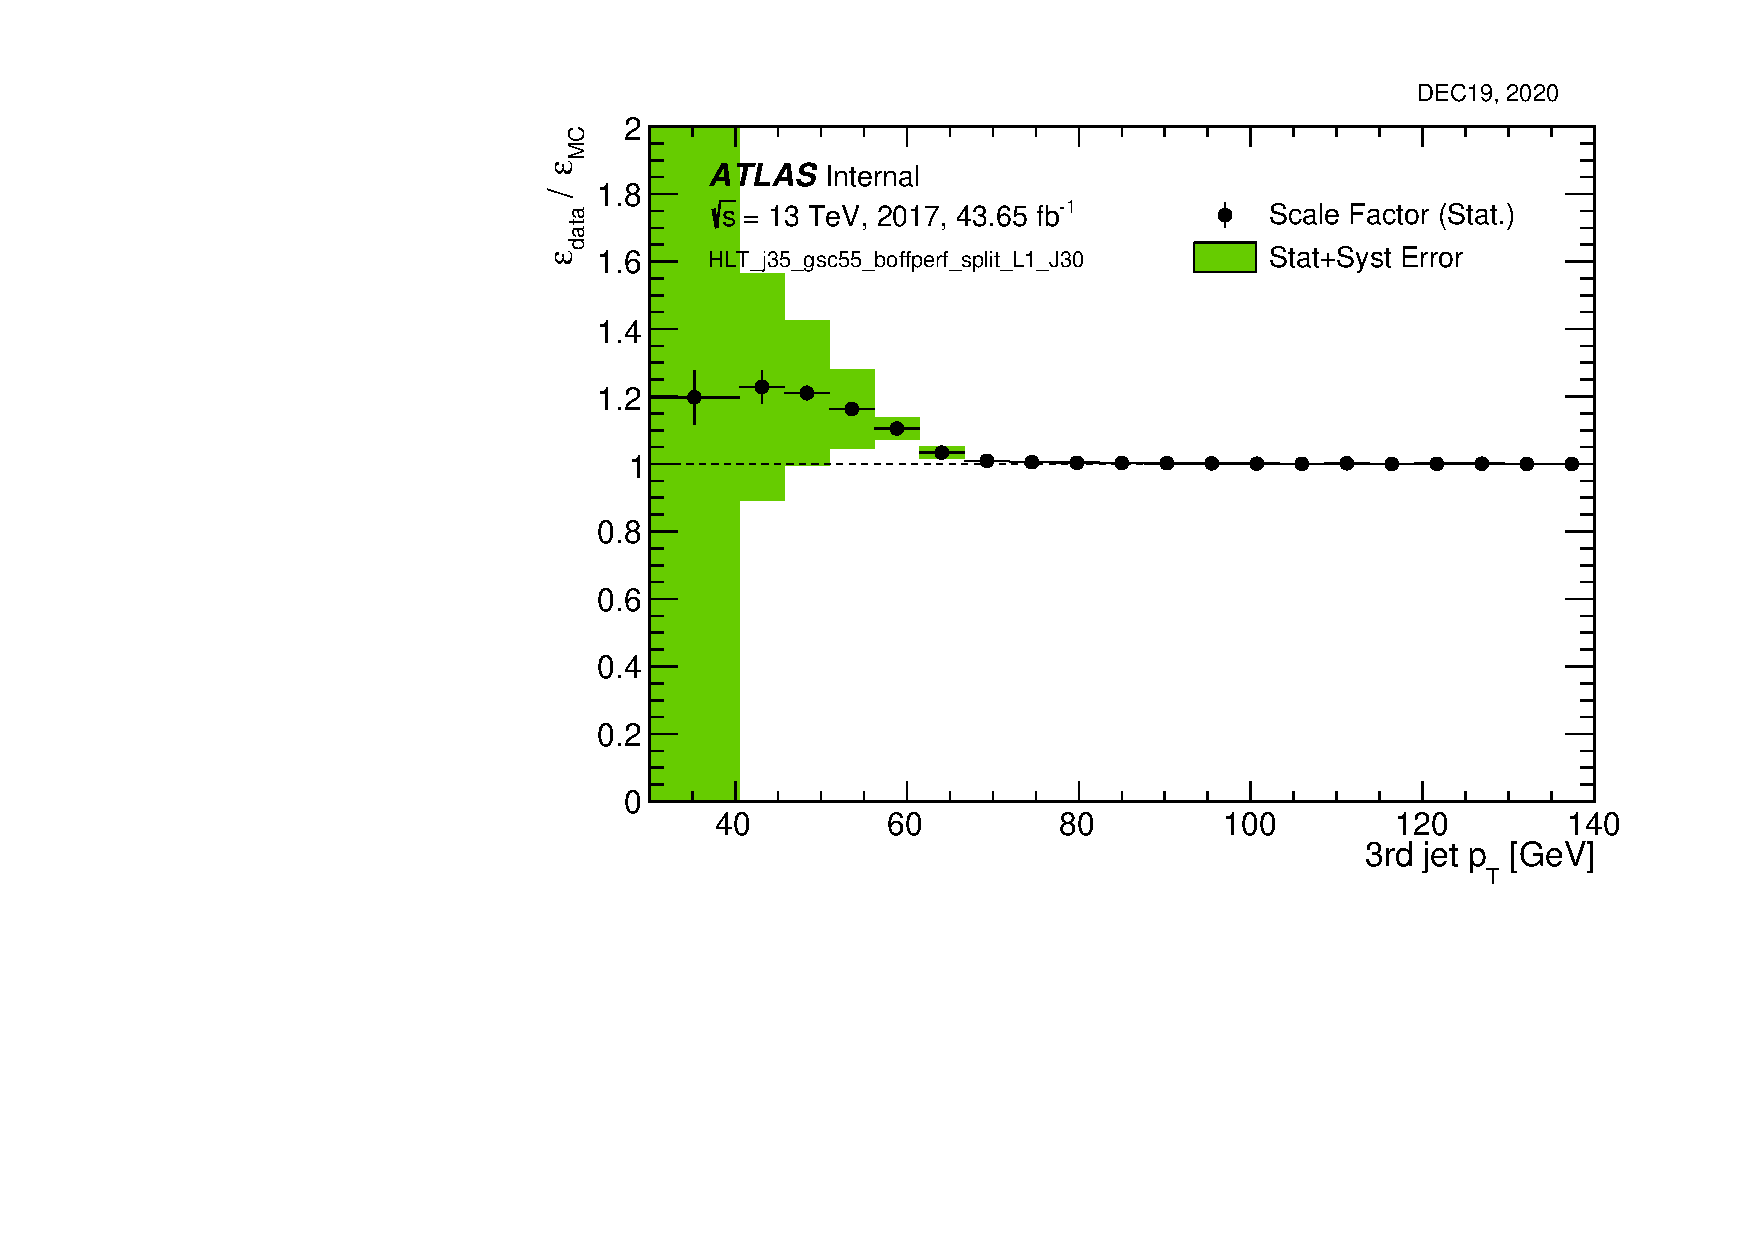
\includegraphics[width=0.3\textwidth]{figures/nr-int-note/appendices/jet-level-trigger-sf/V1/HLTSF/2017/trigSF17-2b1j-HLT-3rd.pdf}
    }

    \caption{Online jet kinematic scale factors of 2b1j trigger as a function of offline jet \pt in 2017. Vertical error bars include statistical uncertainties on the data, while the green bands correspond to the quadrature sum of statistical and systematic uncertainties.}
    \label{fig:jet-kinematict-trigSF17-2b1j}
\end{figure}

%%%%%%%%%%%$%%%
% Trigger definition table
% See defns for the trigger naming convention in:
% https://twiki.cern.ch/twiki/bin/view/Atlas/TriggerNamingRun2#Jet_and_B_jet_Dictionary
% example: 
% https://twiki.cern.ch/twiki/bin/view/Atlas/TrigBjetMenu2017
%
% Seeding for 2b1j 2016 trigger: L15J15
% https://twiki.cern.ch/twiki/bin/view/Atlas/LowestUnprescaled#Bjet_AN2
%%%%%%%%%%%%%%%
%\begin{table}[htbp]
\centering
\begin{tabular}{ccc}
Year                      & Trigger Name                                                                    & \textbf{Trigger Type}  \\ 
\hline
2016 & HLT\_j225\_bmv2c2060\_split                                                     & 1b                     \\
2016                      & HLT\_j100\_2j55\_bmv2c2060\_split                                               & 2b1j                   \\
2016                      & HLT\_2j35\_bmv2c2060\_split\_2j35\_L14J15.0ETA25                                & 2b2j                   \\
2016                      & HLT\_2j55\_bmv2c2060\_split\_ht300\_L14J15                                      & 2bHT                   \\ 
\hline
2017                      & HLT\_j225\_gsc300\_bmv2c1070\_split                                             & 1b                     \\
2017                      & HLT\_j110\_gsc150\_boffperf\_split\_2j35\_gsc55\_bmv2c1070\_split\_L1J85\_3J30  & 2b1j                   \\
2017                      & HLT\_2j15\_gsc35\_bmv2c1040\_split\_2j15\_gsc35\_boffperf\_split\_L14J15.0ETA25 & 2b2j                   \\
2017                      & HLT\_2j35\_gsc55\_bmv2c1050\_split\_ht300\_L1HT190-J15s5.ETA21                  & 2bHT                   \\ 
\hline
2018                      & HLT\_j225\_gsc300\_bmv2c1070\_split                                             & 1b                     \\
2018                      & HLT\_j110\_gsc150\_boffperf\_split\_2j45\_gsc55\_bmv2c1070\_split\_L1J85\_3J30  & 2b1j                   \\
2018                      & HLT\_2j35\_bmv2c1060\_split\_2j35\_L14J15.0ETA25                                & 2b2j                   \\
2018                      & HLT\_2j45\_gsc55\_bmv2c1050\_split\_ht300\_L1HT190-J15s5.ETA21                  & 2bHT                  
\end{tabular}
\caption{Triggers under study for non-resonant searches.}
\label{tab:nr-triggers}
\end{table}


% Redacted text:
%All of these triggers don't have a pre-scale factor, but our analysis is operating on the turn-on curve, as illustrated by \Fig{\ref{fig:HH_trigger_eff}}
%No requirement that the offline jets be ``analysis jets''
% The ``matching efficiency'' is how often we are able to find the online jets in the trigger stream that define the trigger decision, and this is close to 100\% for the six trigger chains under consideration. (Note, this is not saying that the trigger passed, just that we found the online jets to reconstruct what the trigger saw.)
% too detail oriented - if I don't mention it I think the assumption is it is 100%

